\chapter{通信路に減衰がある場合}
今回の評価実験では通信路が減衰の影響を受ける場合について考える。
\figref{Fig:5_1}は減衰の影響について表した。
減衰を受けることにより、平均$\mu$は$\sqrt{k}\mu$となる。
また、共分散行列$A$は、$kA+ (1-k)/4 $となる。ここで、$k$は透過率を表す。ただし、コヒーレント状態の場合、共分散行列は減衰によって変化しない。


\begin{figure}[htbp]
        \centering   
        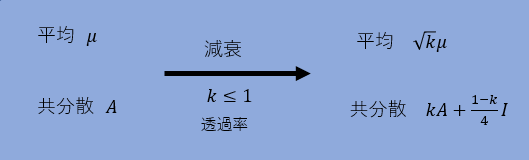
\includegraphics[width=0.8\textwidth]{img/zemi6.png}
        \caption[sample image (png)]{減衰の影響.}
        \label{Fig:5_1}
    \end{figure}





\figref{Fig:5_2}は、今回の評価実験の構成図になる。この通信路が透過率$k$の減衰の影響を受けている。
ここで、送信器の信号の最大強度の設定を$S_{max}$、受信機の信号の最大強度の設定を$S'_{max}$とする。
実験では$S_{max}$と$S´_{max}$が等しい場合と減衰の効果を考慮して$S´_{max}$を決める場合について実験を行った。
また、今回の実験では受信器は乱数を発生させてシミュレートした。
\begin{figure}[H]
        \centering   
        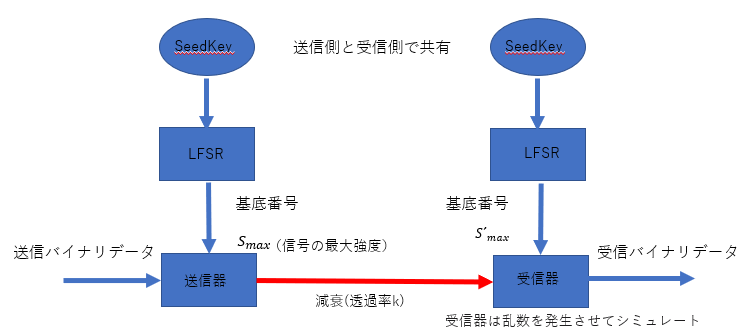
\includegraphics[width=1.0\textwidth]{img/zemi7.png}
        \caption[sample image (png)]{減衰がある場合の正規受信者の誤り率.}
        \label{Fig:5_2}
    \end{figure}


\section{評価実験}
減衰がある場合の正規受信者の誤り率を評価する。以下は送信者側のプログラムである。
\begin{lstlisting}[caption=送信者側のプログラム,label=program1]
import numpy as np
import random

register=np.array([1,0,1,0,1,1,0,0,1,1,1,0,0,0,0,1]) #Seed Keyの設定
#@markdown `基底を決めるのに必要なビット数`
N=8 #@param {type: "number"}

#@markdown `出力される信号の個数`
M=1000 #@param {type: "number"}
BNum=2**N 

#@markdown `信号の最大強度`
#信号の最大強度 (信号の強度は0~S_maxで設定される)
S_max=5 #@param {type: "number"}

S_levels=np.linspace(0,S_max,BNum*2) #使用される信号強度の配列
##--------送受信者共通データ----------##
register=np.array([1,0,1,0,1,1,0,0,1,1,1,0,0,0,0,1]) #Seed Keyの設定

#Driverのためのデータを作成
a=np.zeros(N) #要素数8の配列を0で初期化したものをaに代入
input_Data=np.zeros(M) #送信データは常に0と仮定
#input_Data=[0,1,1,0,1,1,1,0,0,1]
output_qstates=[]

for j in range(M): #データ出力のためのループ
  for i in range(N): #LFSRの出力をNビット分だけ配列aに格納している
    SR=(register[10]+register[12]+register[13]+register[15])%2 
    a[i]=register[15] 
    register=np.roll(register,1) 
    register[0]=SR
    ###
  d=0
  p=1
  ###LFSRからの出力をNビットずつまとめて数値(0~BNum-1)に変換し、Mapperの入力としている
  for i in range(N):
    d+=p*a[i]
    p*=2 
  base_id=int(d)
  index=int(input_Data[j])

#if base_id%2==1:
#    index=(index+1)%2
  index=(index+base_id%2)%2

  output_level=S_levels[base_id+BNum*index] #Driverから出力される信号強度
  q_state=Qstate(output_level) #送信者から出力される量子状態
  output_qstates.append(q_state)
\end{lstlisting}

\begin{lstlisting}[caption=減衰のプログラム,label=program2]
att_rate_total=0.05 #@param {type: "number"}

att_rate=att_rate_total
for j in range(M):
  output_qstates[j].attenuate(att_rate)
\end{lstlisting}

\begin{lstlisting}[caption=受信側のプログラム(最大強度の調整なし),label=program3]

import numpy as np
import random

register=np.array([1,0,1,0,1,1,0,0,1,1,1,0,0,0,0,1]) #Seed Keyの設定

#N=8 


#M=100 
BNum=2**N 


#信号の最大強度 (信号の強度は0~S_maxで設定される)
#S_max*=np.sqrt(att_rate)  #ここを生かして実行してみる
#S_max=10
def getData(q_state,base_id):
  thld=S_max/(2*BNum-1)*(BNum/2+base_id) #base_idからしきい値を決める
  val=q_state.homodyne(thld)
  #print("val:",val)
  #if base_id%2==1:
  #val=(val+1)%2   ##valの値がそのまま出力する際はbase_idが偶数の時のみ,base_idが奇数の時は0と1が反転する
  val=(val+base_id%2)%2
  return val

S_levels=np.linspace(0,S_max,BNum*2) #使用される信号強度の配列
##--------送受信者共通データ----------##
register=np.array([1,0,1,0,1,1,0,0,1,1,1,0,0,0,0,1]) #Seed Keyの設定

#Driverのためのデータを作成
a=np.zeros(N) #要素数8の配列を0で初期化したものをaに代入
input_Data=np.zeros(M) #送信データは常に0と仮定
output_vals=[]

for j in range(M): #データ出力のためのループ
  for i in range(N): #LFSRの出力をNビット分だけ配列aに格納している
    SR=(register[10]+register[12]+register[13]+register[15])%2 
    a[i]=register[15] 
    register=np.roll(register,1) 
    register[0]=SR
    ###
  d=0
  p=1
  ###LFSRからの出力をNビットずつまとめて数値(0~BNum-1)に変換し、Mapperの入力としている
  for i in range(N):
    d+=p*a[i]
    p*=2 
  base_id=int(d)

  output_vals.append(getData(output_qstates[j],base_id)) #出てきた値に対して配列の要素として持つ
  #output_qstates.append(q_state)
  
  #print("-----")
print(np.sum(output_vals)/M)

\end{lstlisting}

\begin{lstlisting}[caption=受信側のプログラム(最大強度の調整あり),label=program4]


import numpy as np
import random

register=np.array([1,0,1,0,1,1,0,0,1,1,1,0,0,0,0,1]) #Seed Keyの設定

#N=8 


#M=100 
BNum=2**N 


#信号の最大強度 (信号の強度は0~S_maxで設定される)
S_max*=np.sqrt(att_rate)  #ここを生かして実行してみる
#S_max=10
def getData(q_state,base_id):
  thld=S_max/(2*BNum-1)*(BNum/2+base_id) #base_idからしきい値を決める
  val=q_state.homodyne(thld)
  #print("val:",val)
  #if base_id%2==1:
  #val=(val+1)%2   ##valの値がそのまま出力する際はbase_idが偶数の時のみ,base_idが奇数の時は0と1が反転する
  val=(val+base_id%2)%2
  return val

S_levels=np.linspace(0,S_max,BNum*2) #使用される信号強度の配列
##--------送受信者共通データ----------##
register=np.array([1,0,1,0,1,1,0,0,1,1,1,0,0,0,0,1]) #Seed Keyの設定

#Driverのためのデータを作成
a=np.zeros(N) #要素数8の配列を0で初期化したものをaに代入
input_Data=np.zeros(M) #送信データは常に0と仮定
output_vals=[]

for j in range(M): #データ出力のためのループ
  for i in range(N): #LFSRの出力をNビット分だけ配列aに格納している
    SR=(register[10]+register[12]+register[13]+register[15])%2 
    a[i]=register[15] 
    register=np.roll(register,1) 
    register[0]=SR
    ###
  d=0
  p=1
  ###LFSRからの出力をNビットずつまとめて数値(0~BNum-1)に変換し、Mapperの入力としている
  for i in range(N):
    d+=p*a[i]
    p*=2 
  base_id=int(d)

  output_vals.append(getData(output_qstates[j],base_id)) #出てきた値に対して配列の要素として持つ
  #output_qstates.append(q_state)
  
  #print("-----")
print(np.sum(output_vals)/M)

\end{lstlisting}



\figref{Fig:5_4}は信号の最大強度が5、基底数が256、送信データ数が1000個の場合に透過率と正規受信者の誤り率の関係を表したものである。また、縦軸は誤り率、横軸は透過率で、透過率を0〜0.05づつ1.0まで上げた際の変化をまとめた。グラフからわかる通り、信号の最大強度を調整することで、0.05〜0.6の間で誤り率を大幅に減らすことができることがわかる。また透過率が0.8~1.0の範囲では信号の最大強度を調整しなくても信号の誤り率が低くなることがわかる。

\begin{figure}[htbp]
        \centering   
        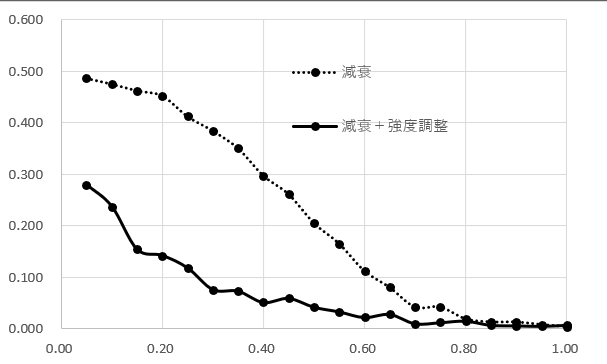
\includegraphics[width=1\textwidth]{img/zemi16.png}
        \caption[sample image (png)]{透過率と正規受信者の誤り率の関係.}
        \label{Fig:5_4}
    \end{figure}